%!TEX TS-program = ../make.zsh

\begin{frame}[fragile]{Project status}

  \begin{columns}
    \begin{column}{0.5\textwidth}
      \begin{overlayarea}{\textwidth}{\textheight}
        \begin{itemize}
          \item<alert@1>[\done] Implement new ray-tracing algorithm
          \item<alert@2>[\done] Implement hole ice and cables
          \item<alert@3>[\done] Verify plausibility with examples
          \item<alert@4>[\done] Verify with statistical cross checks
          \item<alert@5>[\done] Compare to effective descriptions
          \item<alert@6>[\inprogress] Fix compatibility issues with
          \begin{itemize}
            \item[\inprogress] server-client-architecture rewrite
            \item[\tobedone] ice anisotropy
            \item[\tobedone] Unit-test framework
          \end{itemize}
          \item<alert@7>[\tobedone] Implement detection-probability property
          \item<alert@8>[\tobedone] Provide ready-to-use mDOM and D-Egg
          \item<alert@9>[\tobedone] Provide python-3 example scripts \& documentation
        \end{itemize}
      \end{overlayarea}
    \end{column}
    \begin{column}{0.5\textwidth}%
      \only<1>{\image{how-does-it-work-004}}%
      \only<2>{\image{cable-inside-shifted-bc-steamshovel}}%
      \only<3>{
        \begin{center}
          %\hspace{10mm}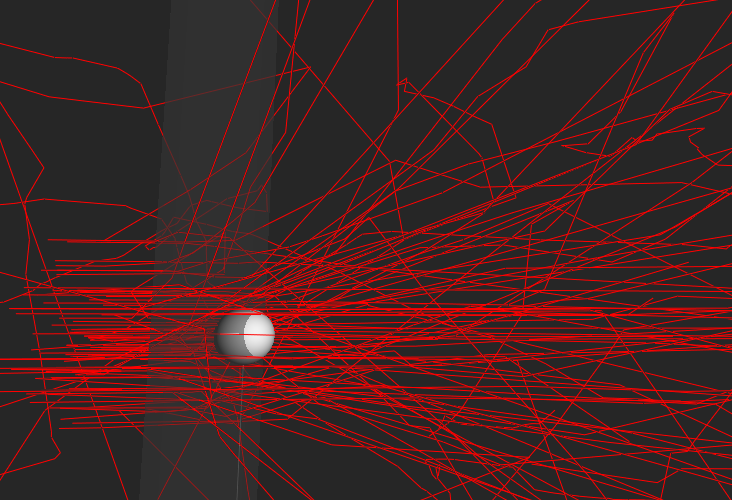
\includegraphics[width=0.8\textwidth]{img/asymmetry-example-steamshovel}
          %\image{asymmetry-example-angular-acceptance-with-comment}
          \vspace*{-1cm}
          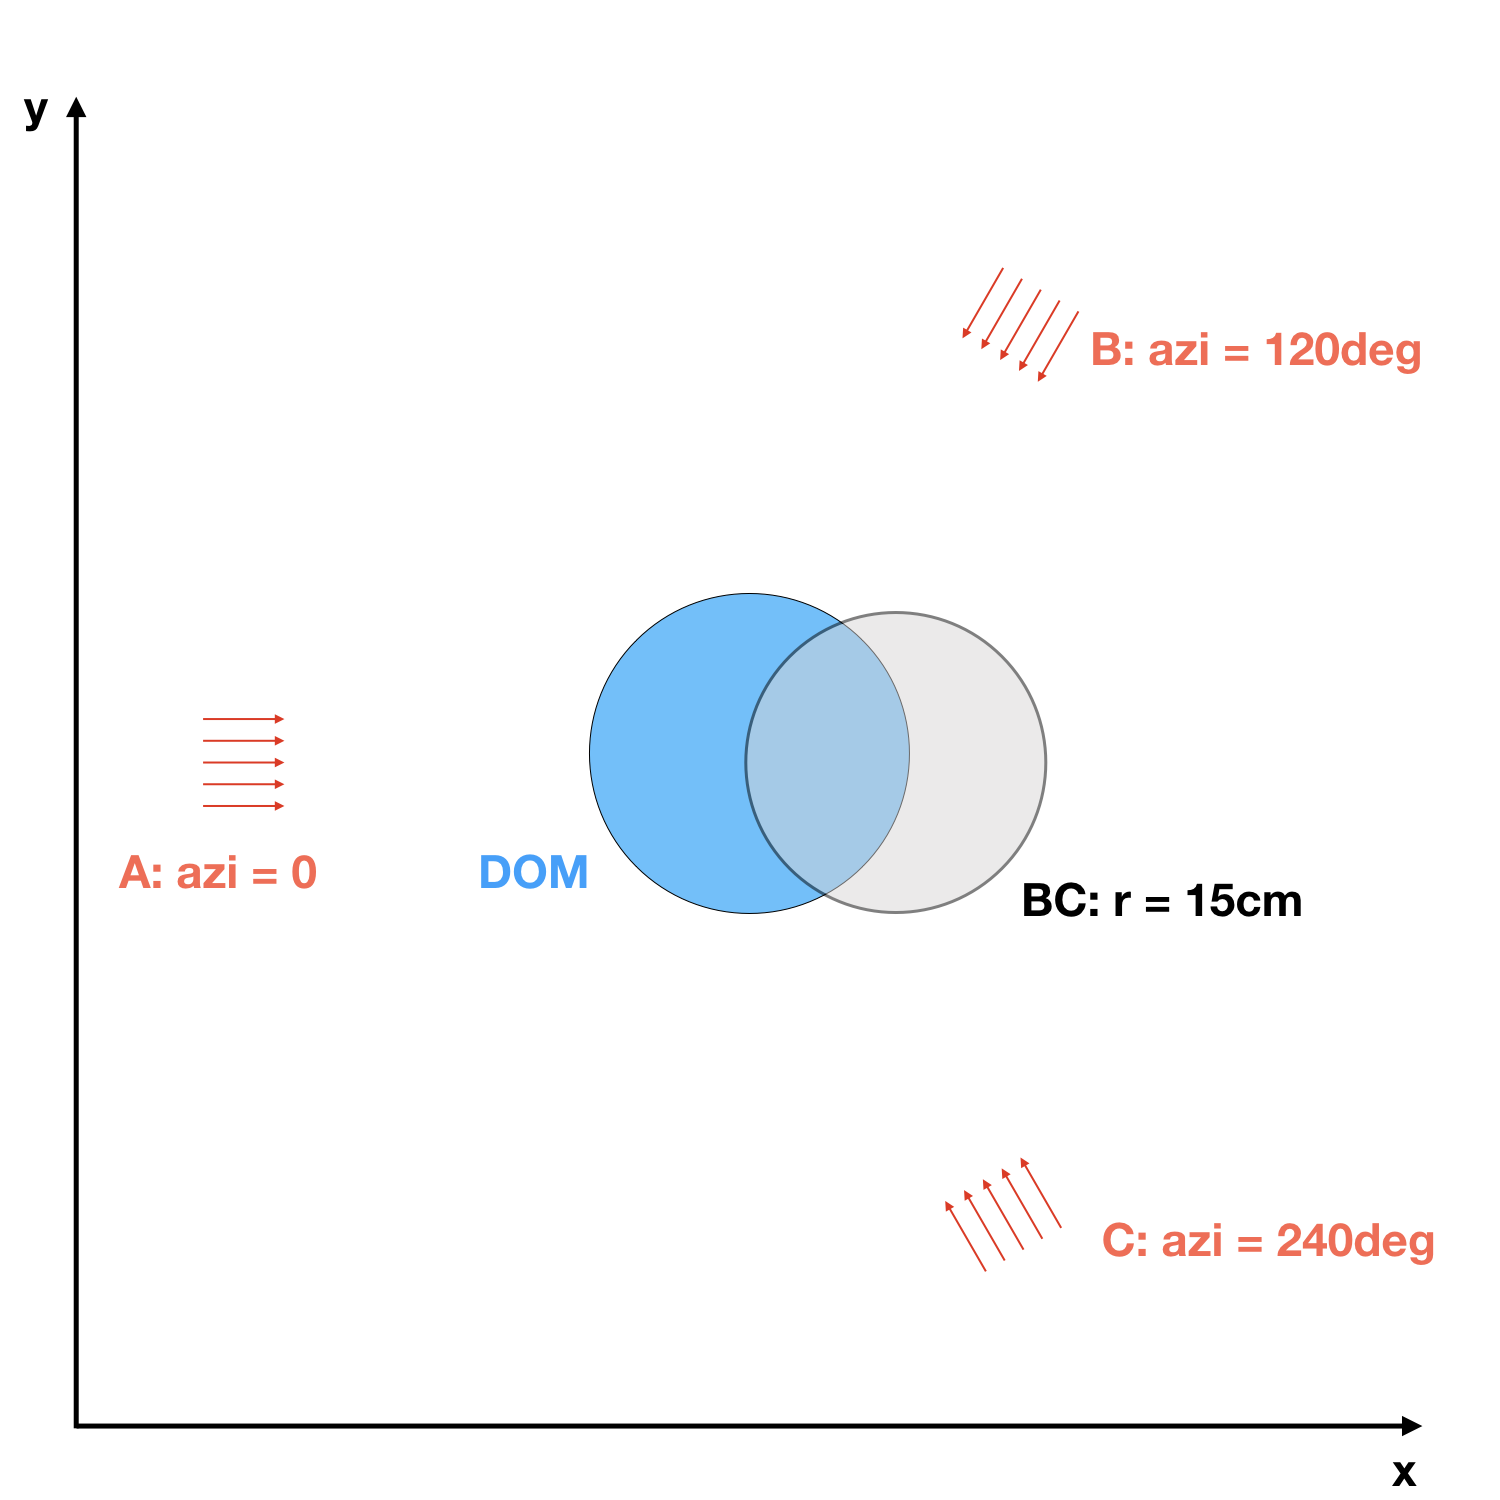
\includegraphics[width=0.6\textwidth]{img/summerscenario-004}
          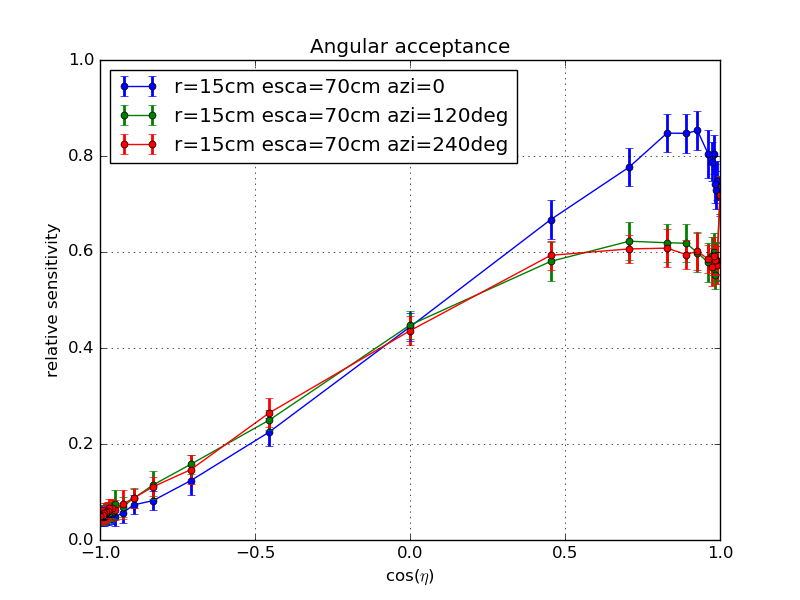
\includegraphics[width=0.8\textwidth]{img/summer_scenario_r15cm_esca70cm}
        \end{center}
      }%
      \only<4>{
        \image{cross-check-66-path-length-histogram}

        \tiny See also: \url{https://github.com/fiedl/hole-ice-study/issues/66}
      }%
      \only<5>{
        \image{ppc-pocam-3}

        \tiny See also: \url{https://github.com/fiedl/hole-ice-study/issues/4}, \url{https://github.com/fiedl/hole-ice-study/labels/comparison}

        \normalsize
        \vspace{2em}

        \metroset{block=fill}
        \begin{block}{Thesis \& previous talks}
          %$\rightarrow$ Thesis \& previous talks: \\
          \url{https://arxiv.org/abs/1904.08422} \\
          \scriptsize \url{https://github.com/fiedl/hole-ice-talk/releases}
        \end{block}

      }%
      \only<6>{Currently resolving technical issues due to major rewrite of the underlying tool.}%
      \only<7-8>{Next step: For ray-tracing, each geometric object (cylinders, spheres, \dots) can have a probability to detect the photon on interaction (absorption, scattering). This can be used to model the photo-sensitive areas of a detector module.}
      \only<8>{
        \vspace{1em}
        Then: Read detector-module type from simulation configuration and place corresponding preset at the position of the module.

        \centering\vspace{1em}
        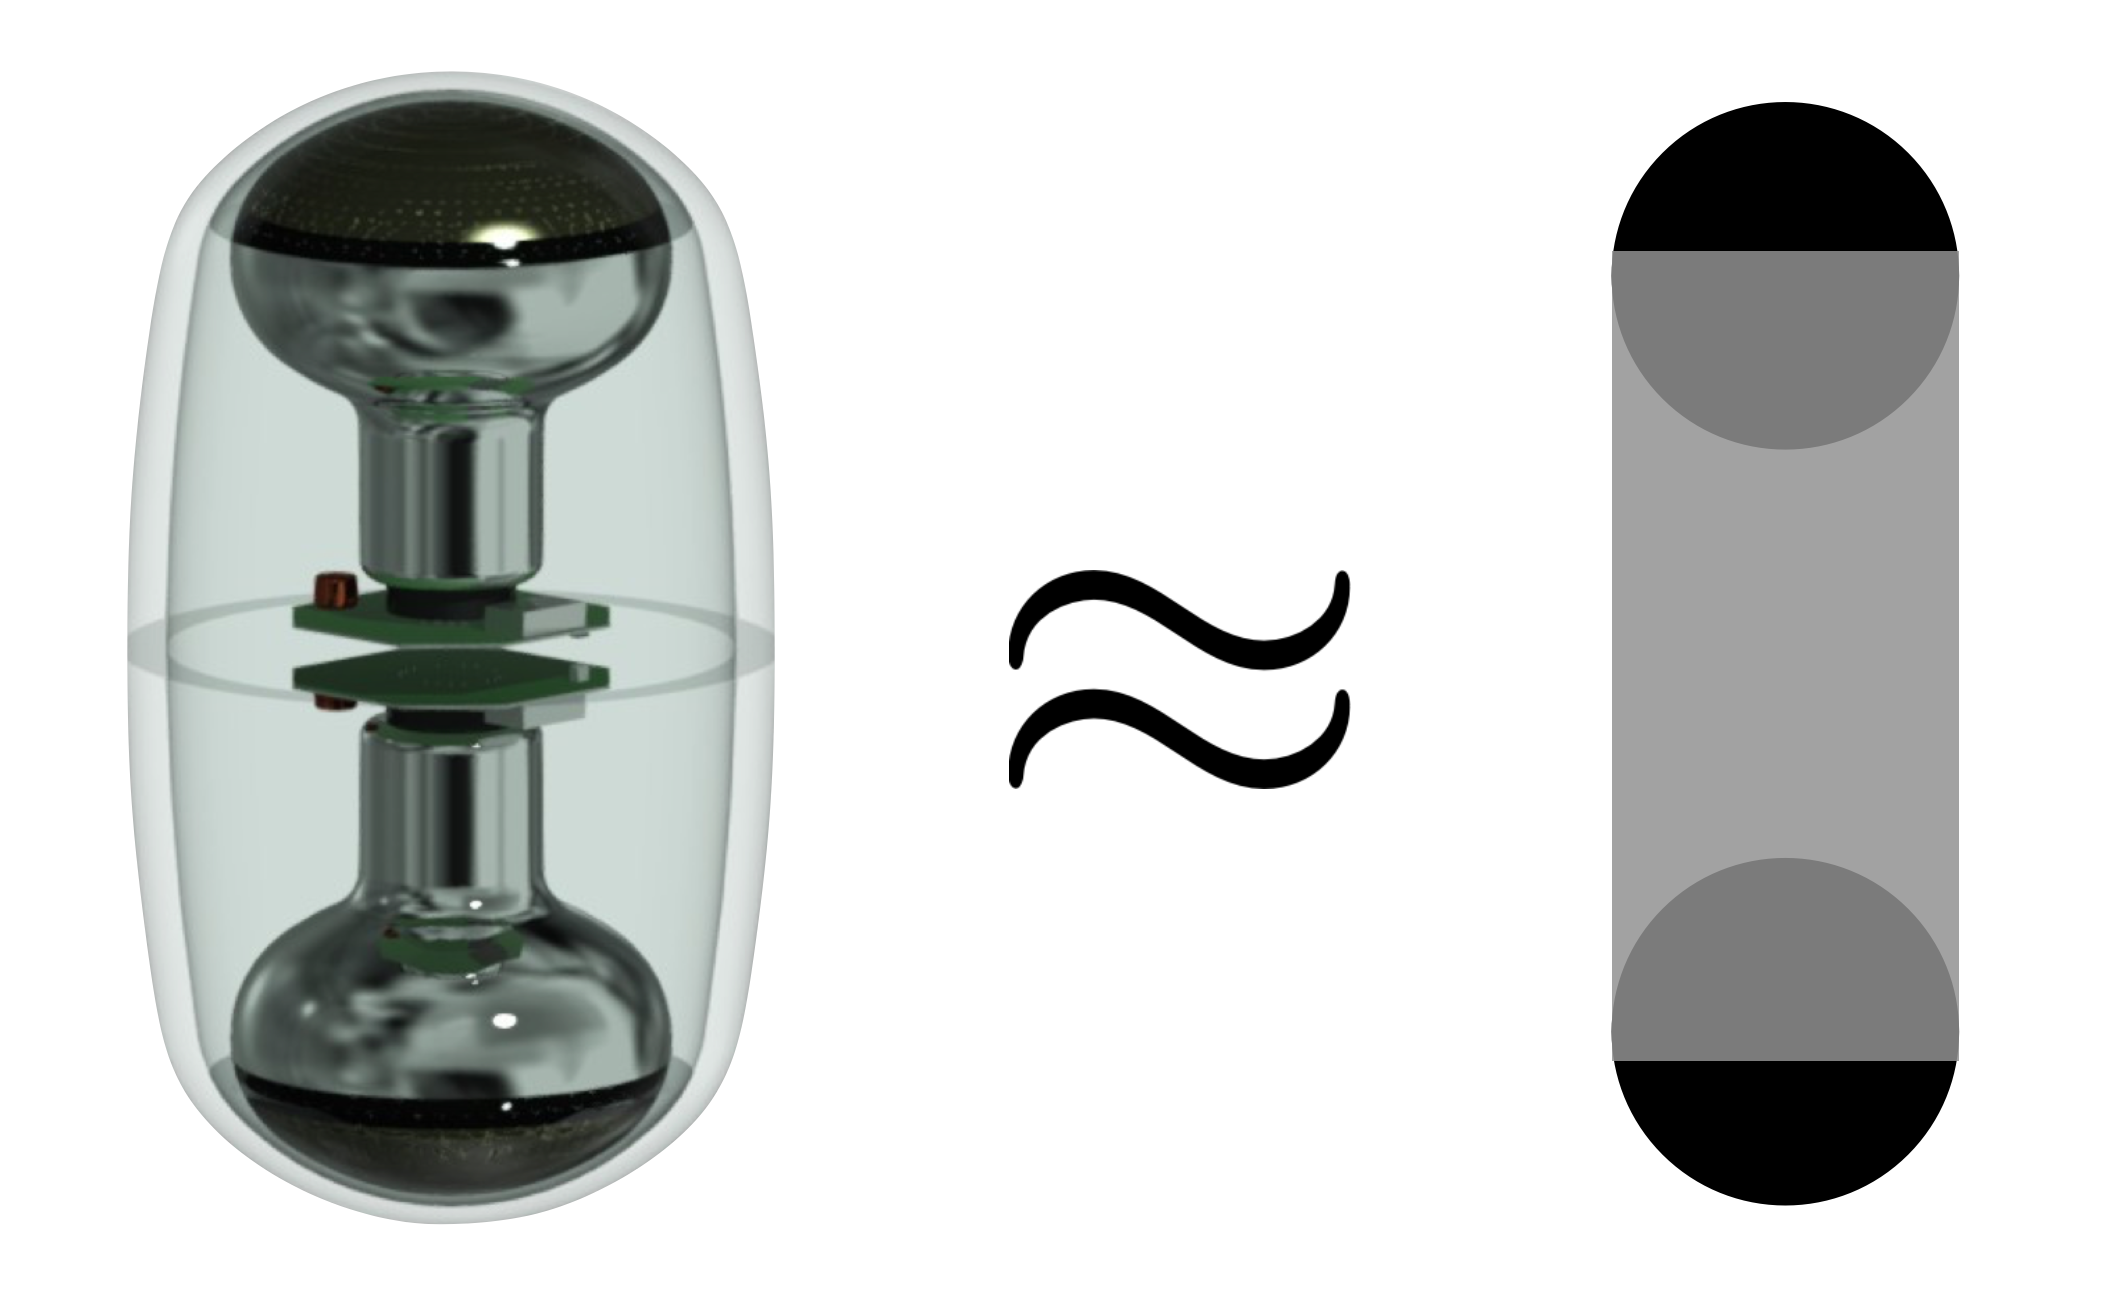
\includegraphics[width=0.8\textwidth]{img/d-egg_approximation}
      }
    \end{column}
  \end{columns}

\end{frame}